\documentclass[border=8pt]{standalone}
\usepackage[T1]{fontenc}\usepackage{lmodern}\usepackage{amsmath}\usepackage[dvipsnames]{xcolor}
\usepackage{tikz}\usetikzlibrary{positioning,arrows.meta,fit,backgrounds,calc,shapes.geometric}
% ---- colours of the system diagrams (one per MQTT topic / kind of traffic)
\definecolor{cSensor}{RGB}{37,99,235}     % sensors/<node>
\definecolor{cAlert}{RGB}{220,38,38}      % ids/alerts
\definecolor{cStats}{RGB}{22,163,74}      % ids/stats
\definecolor{cMit}{RGB}{124,58,237}       % ids/mitigation/status
\definecolor{cStatus}{RGB}{100,116,139}   % ids/status
\definecolor{cCmd}{RGB}{234,88,12}        % cmd/mitigation
\definecolor{cAttack}{RGB}{153,27,27}     % attack traffic
\definecolor{cBot}{RGB}{161,98,7}         % bot master commands (UDP, not MQTT)
\definecolor{cPi}{RGB}{220,38,90}
\definecolor{cLap}{RGB}{51,65,85}
\definecolor{cNode}{RGB}{8,145,178}
\newcommand{\topicdot}[1]{\textcolor{#1}{\rule{0.9em}{0.9em}}}

\tikzset{
  box/.style={draw=#1!70!black, fill=#1!8, rounded corners=4pt, align=center, font=\small, line width=0.7pt,
              inner sep=6pt},
  box/.default=gray,
  group/.style={draw=#1, rounded corners=8pt, line width=1.1pt, inner sep=10pt},
  grouplabel/.style={font=\bfseries\small, text=#1, fill=white, inner sep=3pt},
  pub/.style={-{Stealth[length=7pt]}, line width=1.3pt, draw=#1},
  deliver/.style={-{Stealth[length=7pt]}, line width=1.3pt, draw=#1, dashed},
  attack/.style={-{Stealth[length=8pt]}, line width=1.8pt, draw=cAttack, densely dashed},
  botcmd/.style={-{Stealth[length=7pt]}, line width=1.3pt, draw=cBot, densely dotted},
  lbl/.style={font=\scriptsize\ttfamily, text=#1, fill=white, inner sep=1.5pt},
  flow/.style={-{Stealth[length=6pt]}, line width=1pt, draw=gray!70!black},
}

\begin{document}
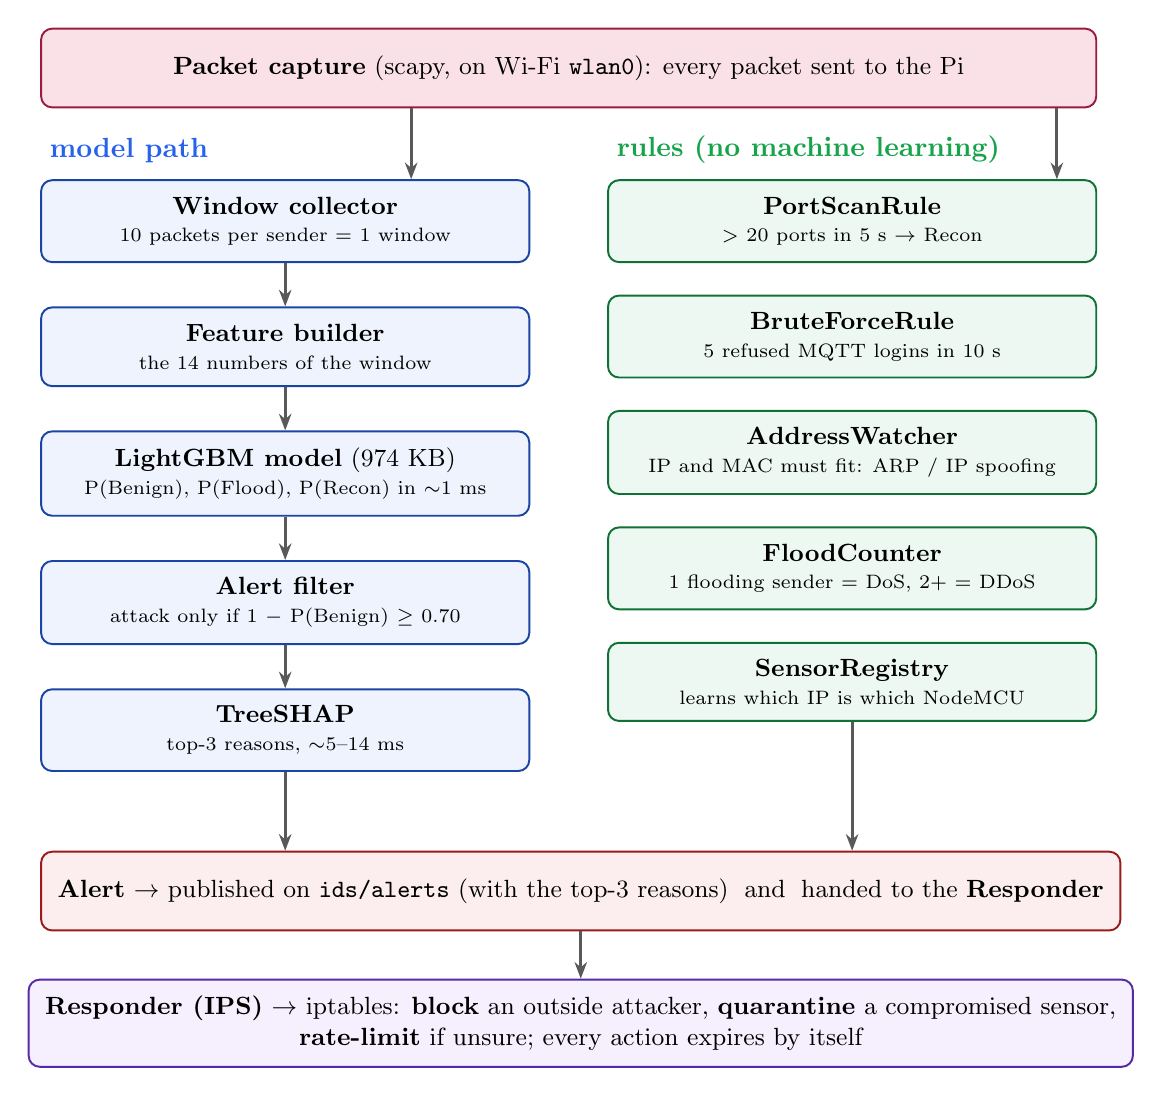
\begin{tikzpicture}[font=\small, node distance=0.55cm]

\node[box=cPi, minimum width=13.4cm, minimum height=1.0cm, fill=cPi!14] (cap)
  {\textbf{Packet capture} (scapy, on Wi-Fi \texttt{wlan0}): every packet sent to the Pi};

\node[box=cSensor, minimum width=6.2cm, minimum height=1.0cm, below=0.9cm of cap.south west, anchor=north west] (win)
  {\textbf{Window collector}\\[-1pt]{\scriptsize 10 packets per sender = 1 window}};
\node[box=cSensor, minimum width=6.2cm, minimum height=1.0cm, below=of win] (feat)
  {\textbf{Feature builder}\\[-1pt]{\scriptsize the 14 numbers of the window}};
\node[box=cSensor, minimum width=6.2cm, minimum height=1.0cm, below=of feat] (lgbm)
  {\textbf{LightGBM model} (974 KB)\\[-1pt]{\scriptsize P(Benign), P(Flood), P(Recon) in $\sim$1 ms}};
\node[box=cSensor, minimum width=6.2cm, minimum height=1.0cm, below=of lgbm] (filt)
  {\textbf{Alert filter}\\[-1pt]{\scriptsize attack only if 1 $-$ P(Benign) $\geq$ 0.70}};
\node[box=cSensor, minimum width=6.2cm, minimum height=1.0cm, below=of filt] (shap)
  {\textbf{TreeSHAP}\\[-1pt]{\scriptsize top-3 reasons, $\sim$5--14 ms}};

\node[box=cStats, minimum width=6.2cm, minimum height=0.85cm, below=0.9cm of cap.south east, anchor=north east] (r1)
  {\textbf{PortScanRule}\\[-1pt]{\scriptsize $>$ 20 ports in 5 s $\rightarrow$ Recon}};
\node[box=cStats, minimum width=6.2cm, minimum height=0.85cm, below=0.4cm of r1] (r2)
  {\textbf{BruteForceRule}\\[-1pt]{\scriptsize 5 refused MQTT logins in 10 s}};
\node[box=cStats, minimum width=6.2cm, minimum height=0.85cm, below=0.4cm of r2] (r3)
  {\textbf{AddressWatcher}\\[-1pt]{\scriptsize IP and MAC must fit: ARP / IP spoofing}};
\node[box=cStats, minimum width=6.2cm, minimum height=0.85cm, below=0.4cm of r3] (r4)
  {\textbf{FloodCounter}\\[-1pt]{\scriptsize 1 flooding sender = DoS, 2+ = DDoS}};
\node[box=cStats, minimum width=6.2cm, minimum height=0.85cm, below=0.4cm of r4] (r5)
  {\textbf{SensorRegistry}\\[-1pt]{\scriptsize learns which IP is which NodeMCU}};

\node[box=cAlert, minimum width=13.4cm, minimum height=1.0cm, below=1.0cm of shap.south west, anchor=north west] (alert)
  {\textbf{Alert} $\rightarrow$ published on \texttt{ids/alerts} (with the top-3 reasons) \;and\; handed to the
  \textbf{Responder}};
\node[box=cMit, minimum width=13.4cm, minimum height=1.0cm, below=0.6cm of alert] (resp)
  {\textbf{Responder (IPS)} $\rightarrow$ iptables: \textbf{block} an outside attacker, \textbf{quarantine} a
  compromised sensor,\\ \textbf{rate-limit} if unsure; every action expires by itself};

\node[font=\bfseries, text=cSensor, anchor=south west] at ($(win.north west)+(0,0.08)$) {model path};
\node[font=\bfseries, text=cStats, anchor=south west] at ($(r1.north west)+(0,0.08)$) {rules (no machine learning)};

\draw[flow] ($(cap.south -| win.north)+(1.6,0)$) -- ($(win.north)+(1.6,0)$);
\draw[flow] ($(cap.south -| r1.north)+(2.6,0)$) -- ($(r1.north)+(2.6,0)$);
\draw[flow] (win) -- (feat); \draw[flow] (feat) -- (lgbm); \draw[flow] (lgbm) -- (filt); \draw[flow] (filt) -- (shap);
\draw[flow] (shap.south) -- (shap.south |- alert.north);
\draw[flow] (r5.south) -- (r5.south |- alert.north);
\draw[flow] (alert) -- (resp);

\end{tikzpicture}
\end{document}
